\documentclass[aspectratio=169]{beamer}

% get rid of clickable beamer buttons
\beamertemplatenavigationsymbolsempty

% parse most utf-8 correctly
\usepackage[utf8]{inputenc}
\usepackage[ngerman]{babel}

% better graphics
\usepackage{graphicx}

% beamer settings
\title{snailmail}
\author{Noah Vogt \& Simon Hammer}
\institute{Gymnasium Kirschgarten}
\usetheme{Copenhagen}

\usepackage{varwidth}

\usepackage{graphicx,calc}
\newlength\myheight
\newlength\mydepth
\settototalheight\myheight{Xygp}
\settodepth\mydepth{Xygp}
\setlength\fboxsep{0pt}

\newcommand*\inlinegraphics[1]{
    \settototalheight\myheight{Xygp}
    \settodepth\mydepth{Xygp}
    \raisebox{-\mydepth}{\includegraphics[height=\myheight]{#1}}%
}

% for code snippits
\usepackage{listings}
\usepackage{color}

\definecolor{dkgreen}{rgb}{0,0.6,0}
\definecolor{gray}{rgb}{0.5,0.5,0.5}
\definecolor{mauve}{rgb}{0.58,0,0.82}
\definecolor{background}{rgb}{0.36,0.36,0.36}

\lstset{
    numbersep=3pt,
    keywordstyle=\color{blue},
    commentstyle=\color{dkgreen},
    stringstyle=\color{mauve},
    breaklines=true,
    numbers=left,
    numberstyle=\scriptsize\color{black},
    frame=none,
    basicstyle = \small\ttfamily,
    breaklines=true
    breakatwhitespace=false,
    columns=flexible,
    xleftmargin=0.5cm,framesep=8pt,framerule=0pt,
    aboveskip=3mm,
    belowskip=3mm,
}

% Package to use videos
\usepackage{movie15}

\begin{document}
\maketitle

\begin{frame}{Inhaltsverzeichniss}
INSERT TOC HERE
\end{frame}

%\section{Vorwort}
\begin{frame}{Motivation}
\begin{varwidth}{.5\textwidth}
        \begin{figure}
            \centering
            
\includegraphics[width=.9\textwidth]{media/macbook.jpg}
        \end{figure}
    \end{varwidth}
    \hfill
    \begin{varwidth}{.5\textwidth}
        \begin{itemize}\pause
            \item allgemeines Interesse\pause
            \item fehlender Edubs-Mail-Client\pause
            %\item fehlender Edubs-Mail-Client\inlinegraphics{media/baslerstab-1.jpg}\pause
            \item persönliche Bedürfnisse
        \end{itemize}
    \end{varwidth} 
\end{frame}

%\subsection{Ziele}
\begin{frame}{Ziele}
\begin{varwidth}{.5\textwidth}
        \begin{figure}
            \centering
            
\includegraphics[width=.8\textwidth]{../logo/version3d.png}
            \caption{snailmail Logo}
        \end{figure}
    \end{varwidth}
    \hfill
    \begin{varwidth}{.5\textwidth}
        \begin{itemize}\pause
            \item Basisfunktionen \inlinegraphics{media/mail.png} \pause
            \item Account Manager\inlinegraphics{media/business.png}\pause
            \item Design Prinzipien\inlinegraphics{media/paintbrush.png}\pause
            \item Schnelligkeit\inlinegraphics{media/run.png}\pause
            \item Mobil und Modern\inlinegraphics{media/mobile.png}\pause
            \item Einstellungen\inlinegraphics{media/settings.png}
        \end{itemize}
    \end{varwidth} 
\end{frame}

\begin{frame}{Warum Java}
\begin{varwidth}{.3\textwidth}
        \begin{figure}
            \centering
            
\includegraphics[height=.8\textheight]{media/java-logo.png}
        \end{figure}
    \end{varwidth}
    \hfill
    \begin{varwidth}{.6\textwidth}
        \begin{itemize}\pause
            \item war offizielle Sprache für Android Apps\pause
            \item abgelöst von Kotlin (seit 2019)\pause
            \item EF Informatik
        \end{itemize}
    \end{varwidth} 
\end{frame}

% TODO: consider using external player
\begin{frame}{Demo}
    INSERT DEMO HERE
    %\includemovie[toolbar]{90pt}{90pt}{media/cutaccountViewer.mp4}
    %\includemovie[]{90pt}{90pt}{media/draftsExample.mp4}
\end{frame}

\begin{frame}{Was alles drin ist}
\includegraphics<1>[height=.8\textheight]{media/emailViewer.jpg}
\pause
\includegraphics<2>[height=.8\textheight]{media/emailWriter.jpg}
\pause
\includegraphics<3>[height=.8\textheight]{media/accountManager.jpg}
\end{frame}

\begin{frame}{allgemeine App-Struktur}
\centering
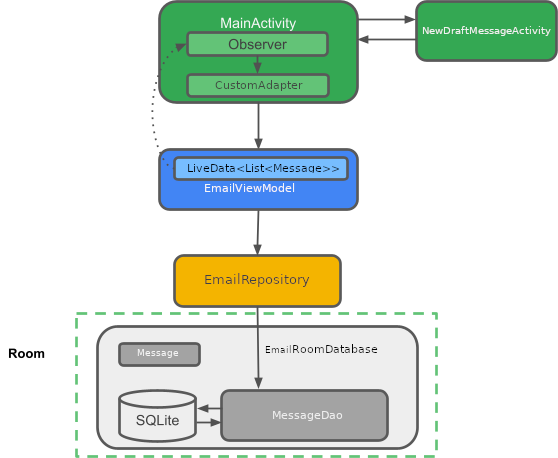
\includegraphics[height=.7\textheight]{../maturText/media/AppStructure.png}
\end{frame}

\begin{frame}{Database}
\begin{block}{allgemein}
\end{block}

\begin{block}{in der app}
\end{block}
\end{frame}

\begin{frame}{Email Connection}
\centering
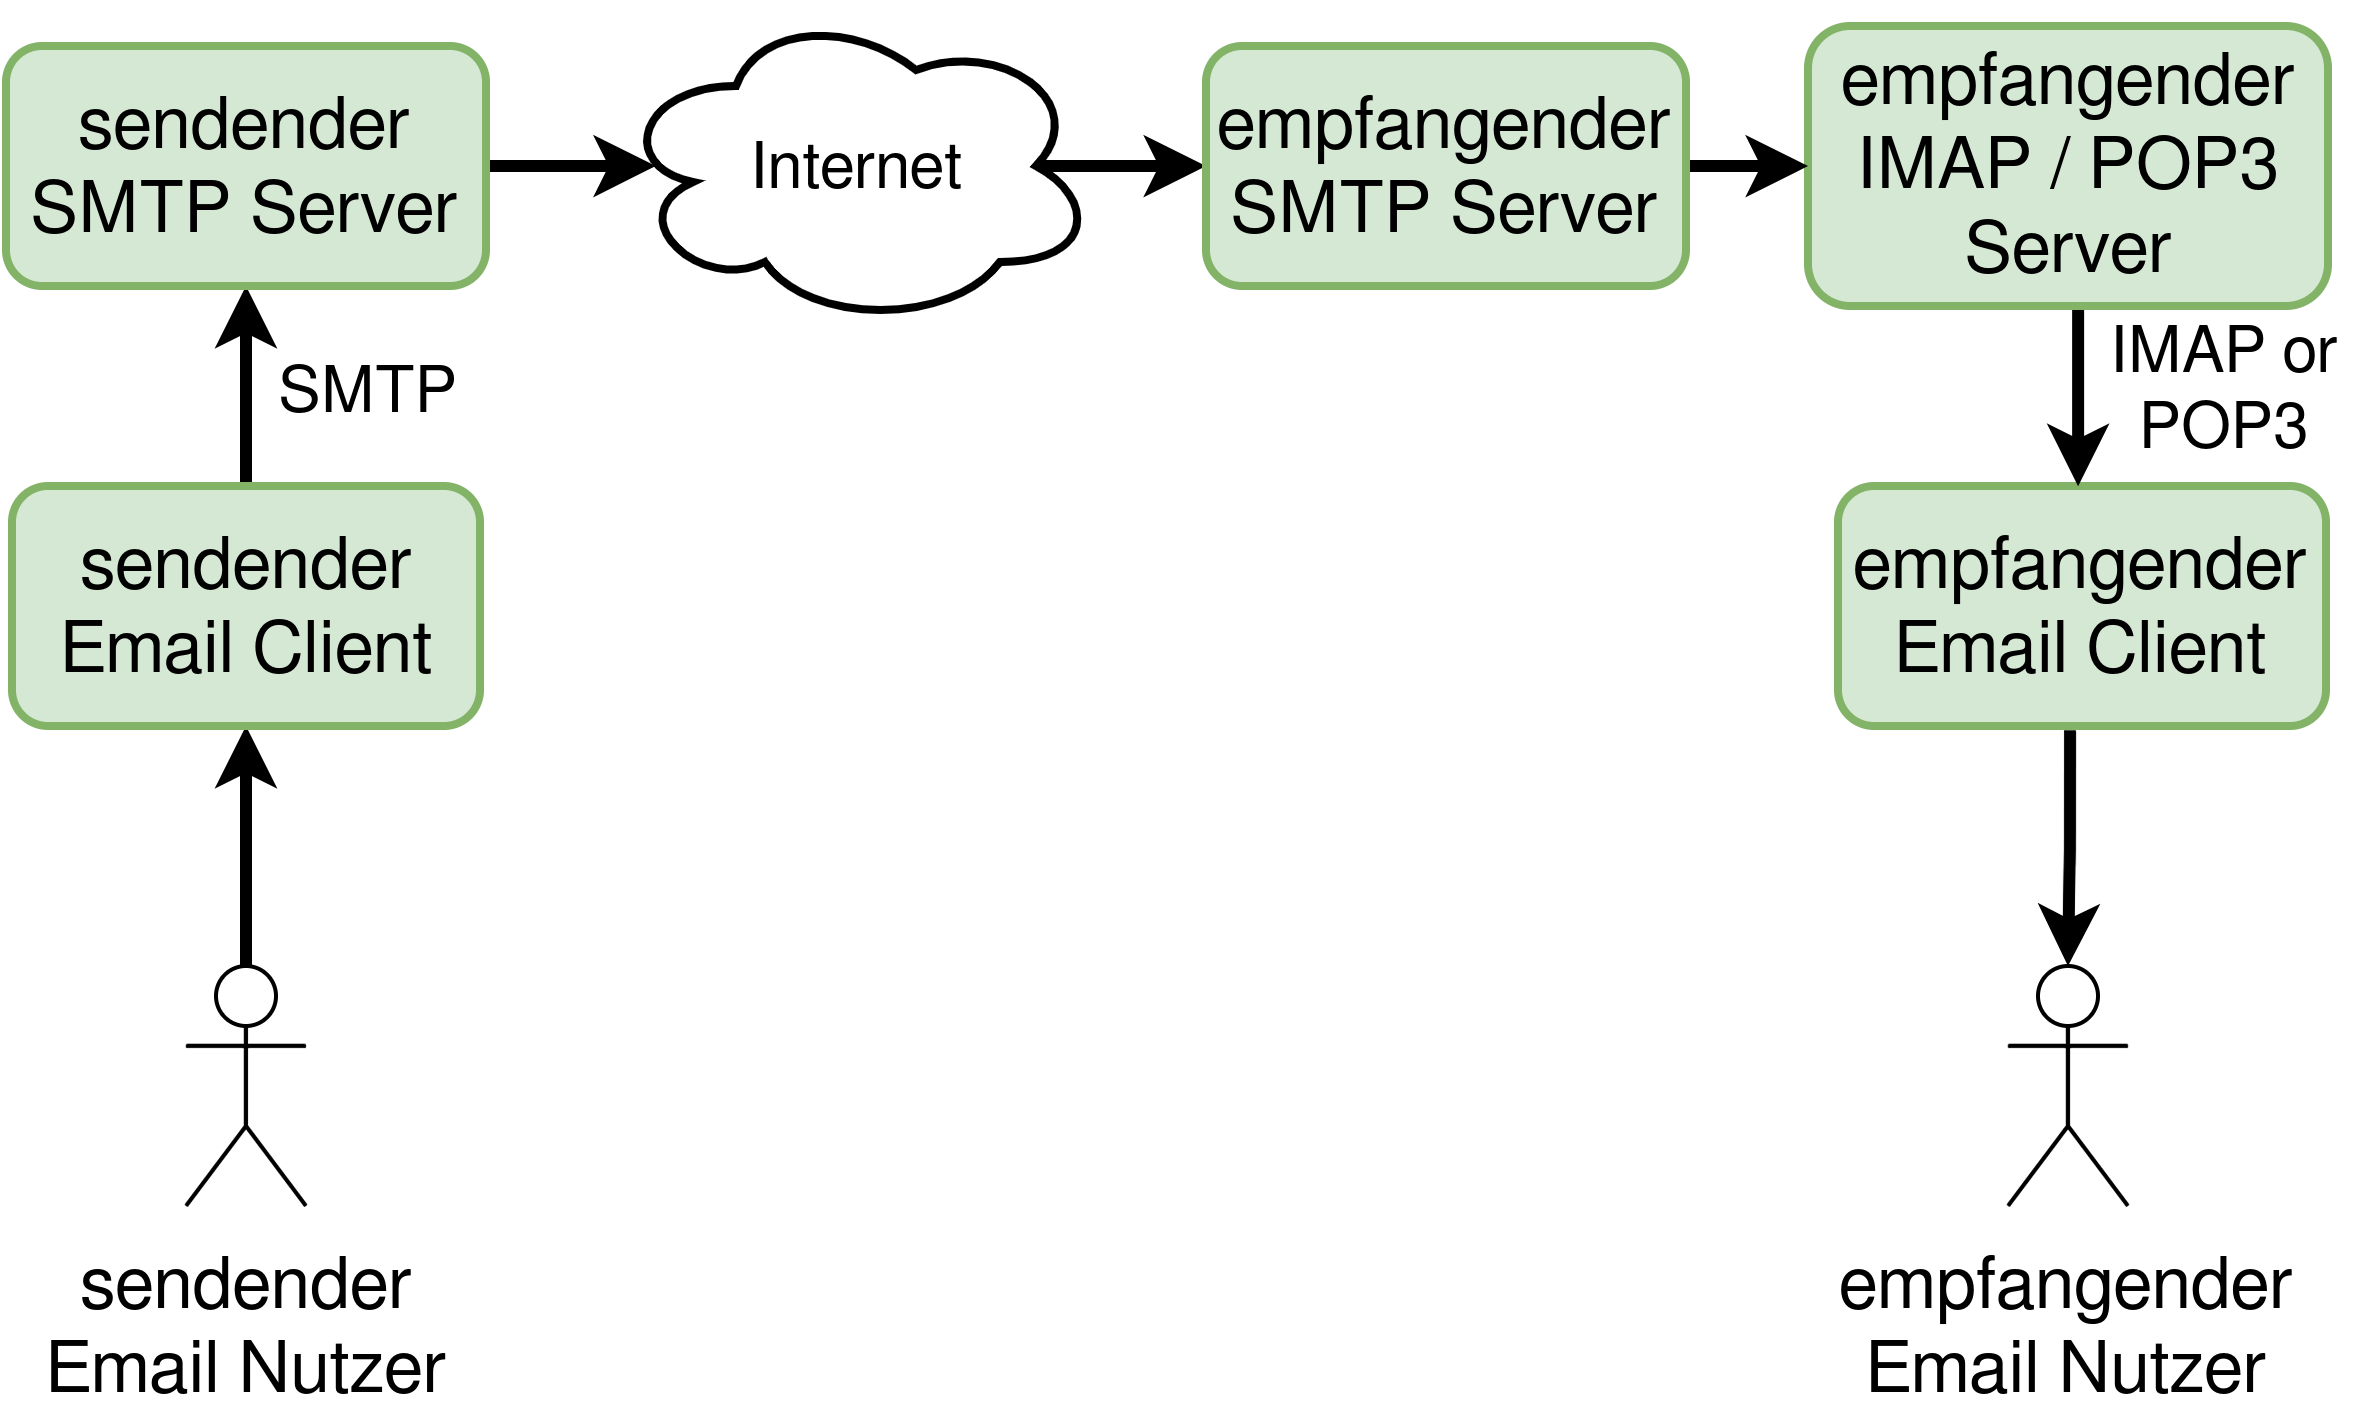
\includegraphics[width=.8\textwidth]{../maturText/media/connection-diagram.png}
\end{frame}

\defverbatim[colored]\makeset{
\lstset{language=python}
\begin{lstlisting}
def sendStarttls(host, sendingMail, receivingMail, password, message="",
                 subject="", port=587, cc=[], bcc=[]):
    context = ssl.create_default_context()

    if type(cc) is not str:
        cc = ",".join(cc)
    if type(bcc) is not str:
        bcc = ",".join(bcc)
    utf8Message = ("Subject: " + subject + "\nCC: " + cc + "\nBCC: " + bcc +
                   "\n\n" + message)
    decoded = utf8Message.encode('cp1252').decode('utf-8')

    with smtplib.SMTP(host, port) as serverConnection:
        serverConnection.starttls(context=context)
        serverConnection.login(sendingMail, password)
        serverConnection.sendmail(sendingMail, receivingMail, decoded)
\end{lstlisting}
}

\begin{frame}{Sendung einer Email}
\makeset
\end{frame}

\begin{frame}{Was haben wir wirklich selber gemacht?}
\centering
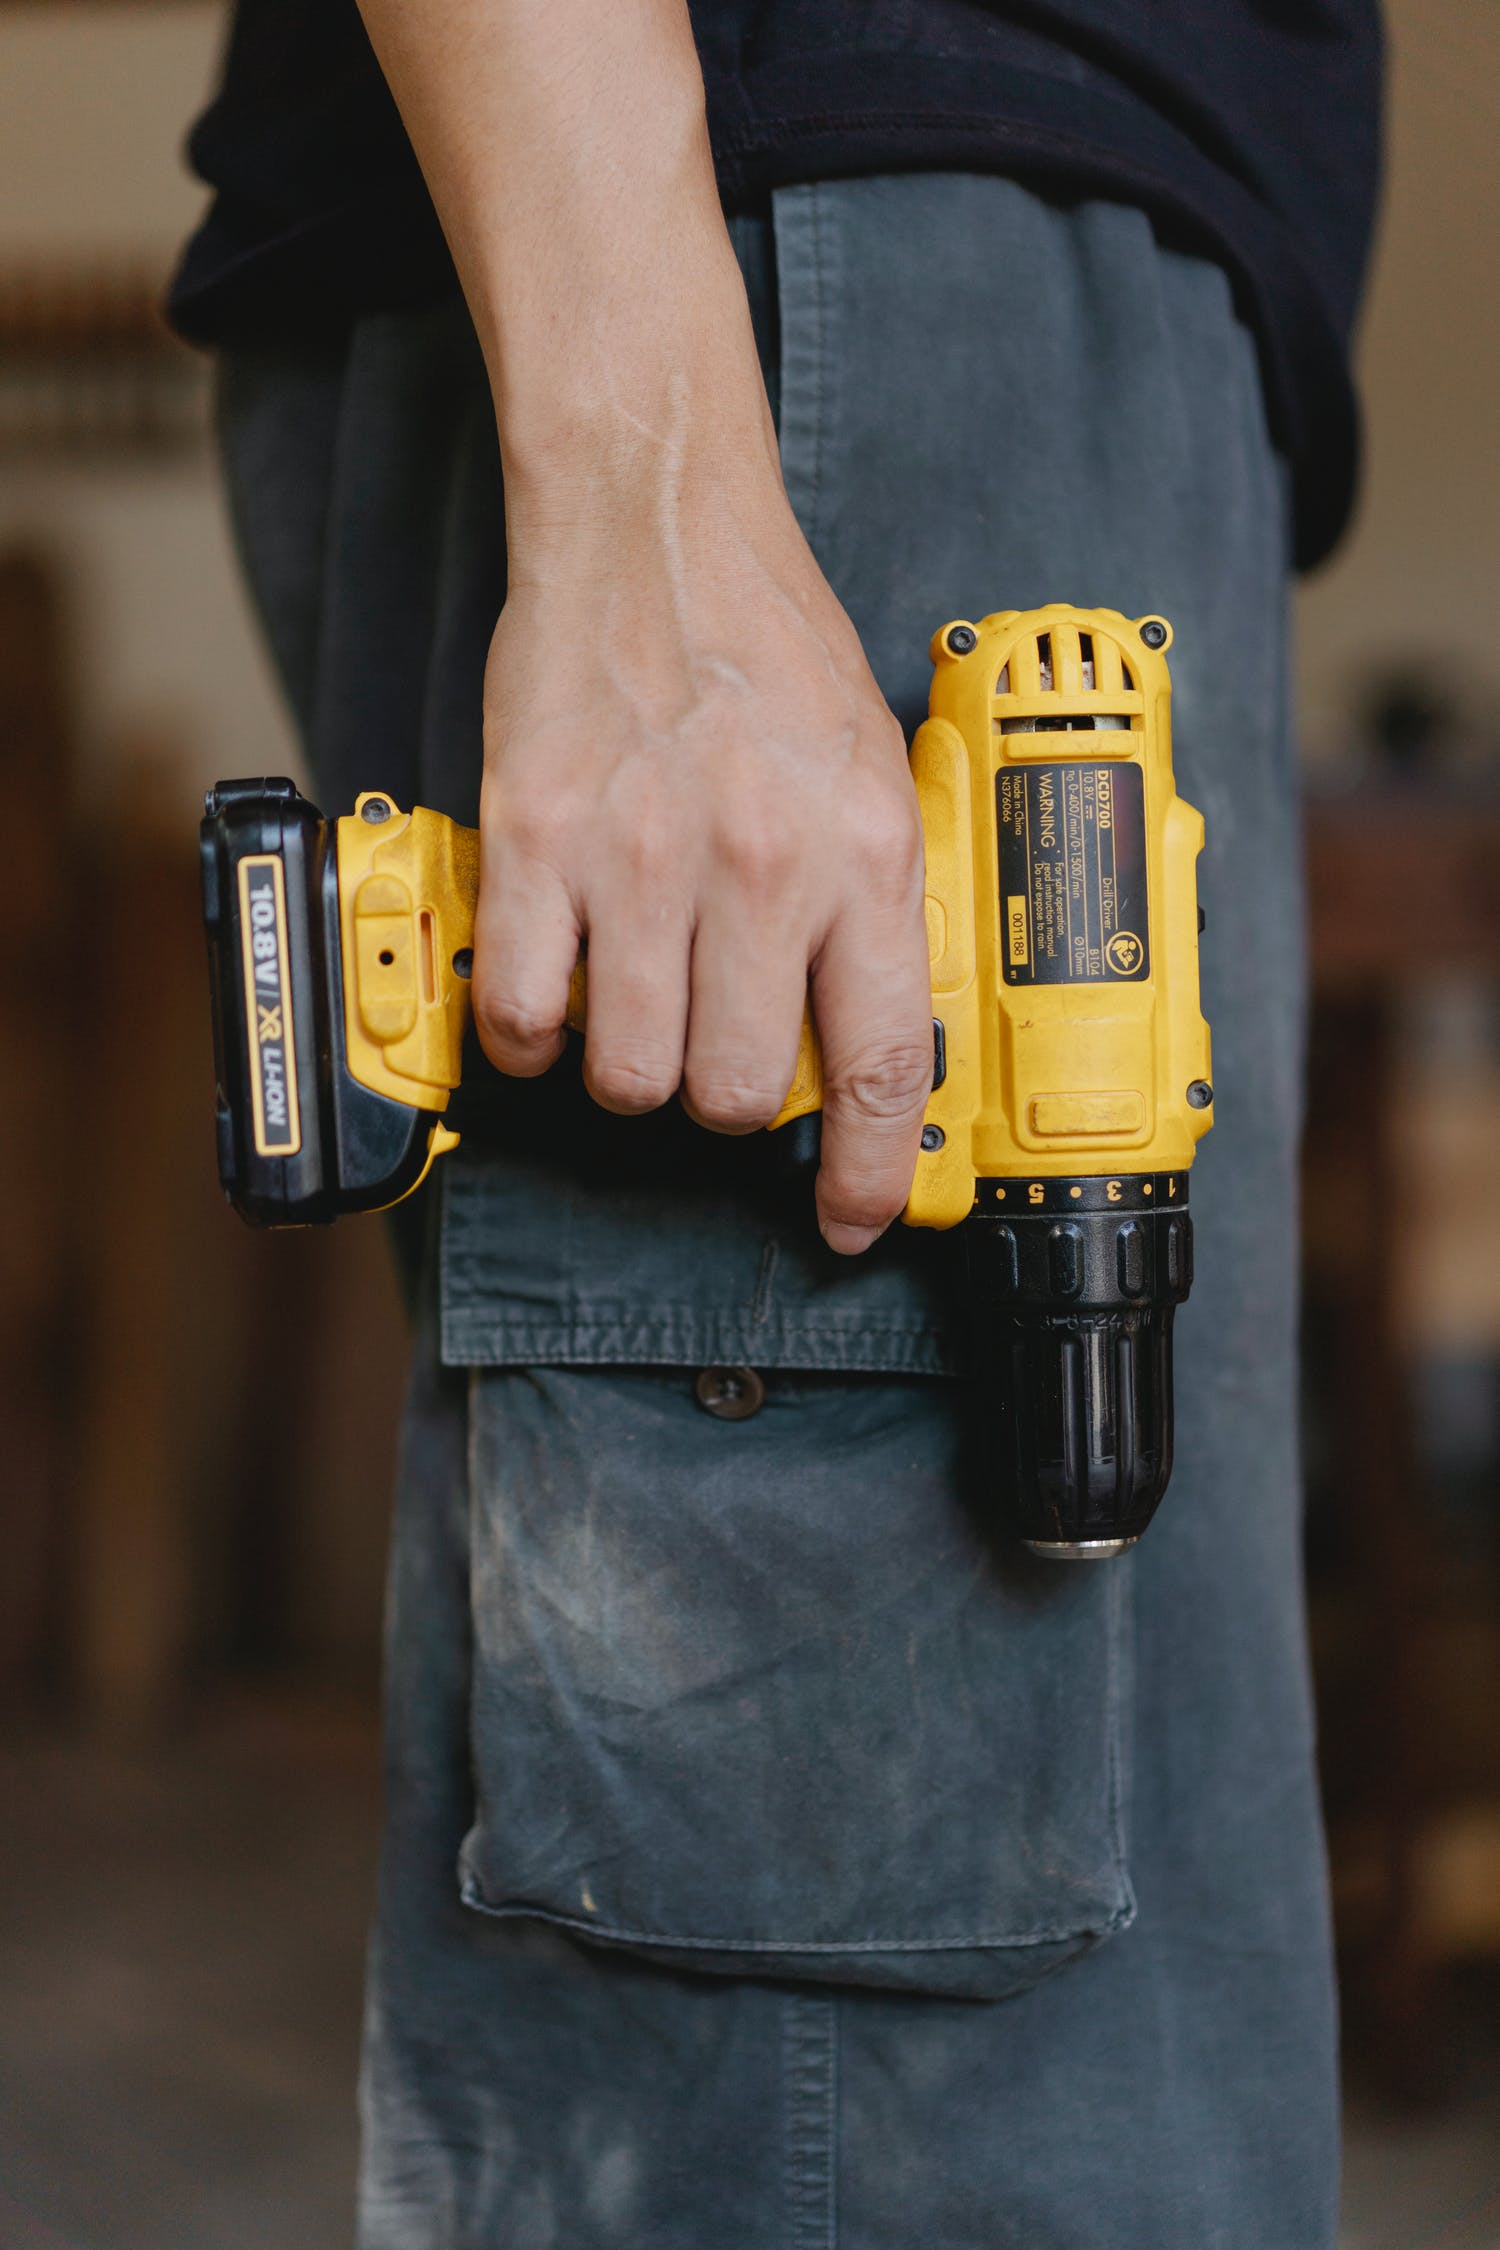
\includegraphics[height=.8\textheight]{media/self.jpeg}
\end{frame}

\begin{frame}{Room}
INSERT ABSTRACTION LAYERS
\end{frame}

\begin{frame}{Material Design}
\begin{varwidth}{.5\textwidth}
        \begin{figure}
            \centering
            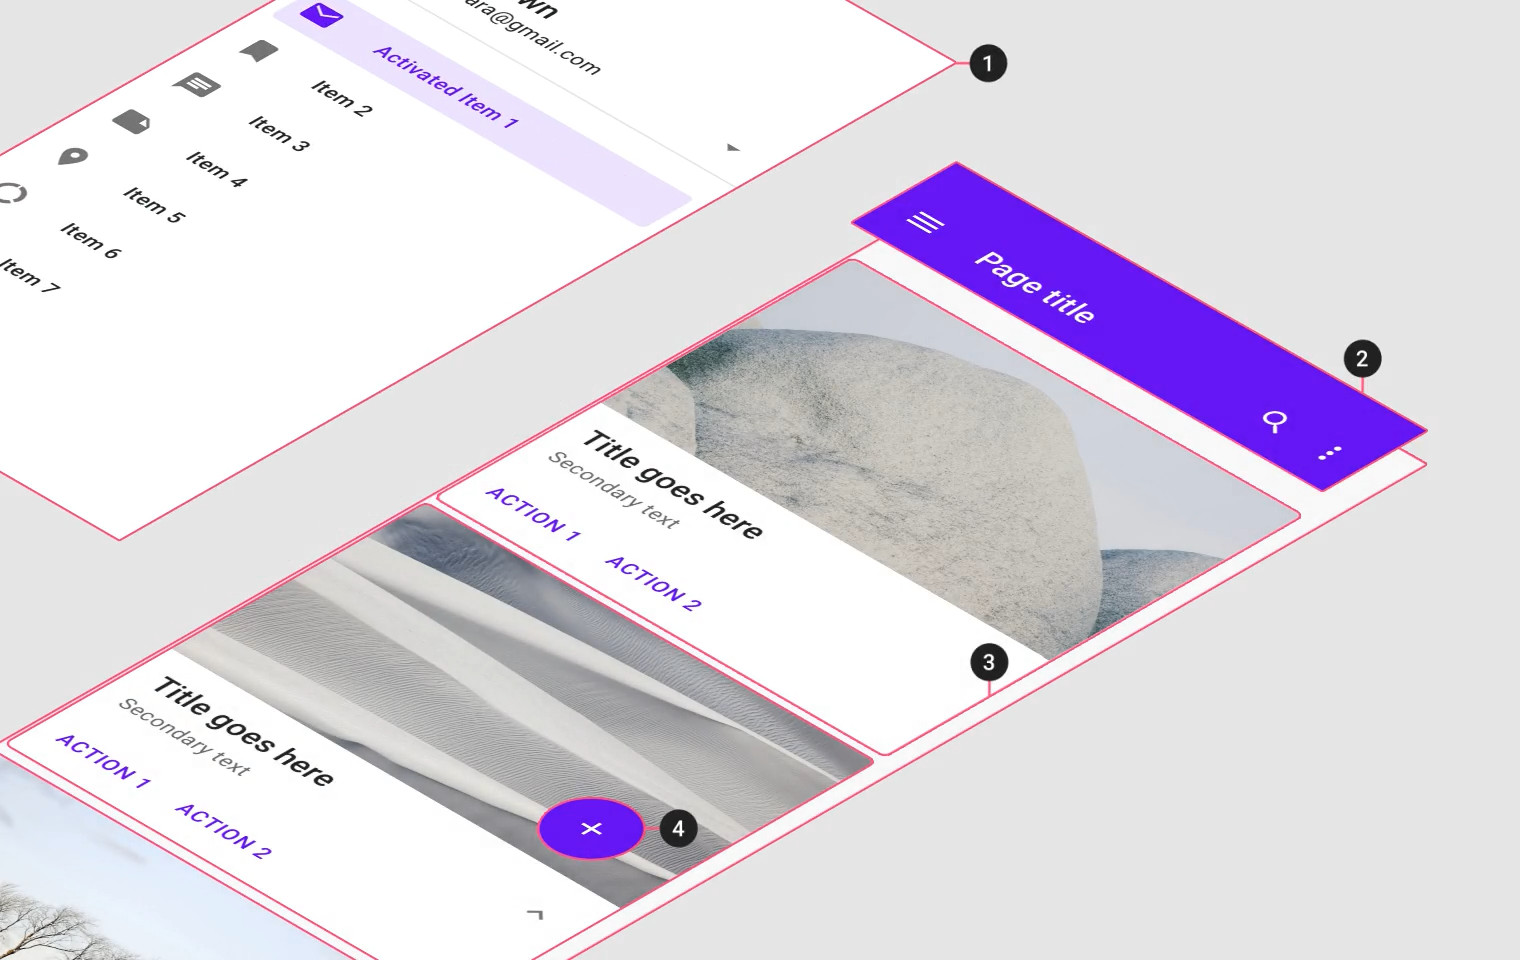
\includegraphics[width=\textwidth]{media/material-design-in-action.jpg}
        \end{figure}
    \end{varwidth}
    \hfill
    \begin{varwidth}{.4\textwidth}
        
\includegraphics[width=\textwidth]{media/material-android.png}
        \begin{itemize}\pause
            \item GUI-Framework\pause
            \item beliebt\pause
            \item in Google Apps
        \end{itemize}
    \end{varwidth}
\end{frame}

\begin{frame}{Bugs}
INSERT BUGS HERE
\end{frame}

%:TODO Ich han eig gmeint Bilder us de Apps. Also wenn du seisch es isch zu überlade das me das in de Apps seht und ned s Logo fo de App
\begin{frame}{Inspiration Design}
\begin{varwidth}{.3\textwidth}\pause
        \begin{figure}
            \centering
            
\includegraphics[width=.9\textwidth]{media/gmail-logo.png}
        \end{figure}
    \end{varwidth}
    \hfill
    \begin{varwidth}{.3\textwidth}\pause
        \begin{figure}
        \centering
        
\includegraphics[width=.9\textwidth]{media/k9-logo.png}
        \end{figure}
    \end{varwidth}
    \hfill
    \begin{varwidth}{.3\textwidth}\pause
        \begin{figure}
        \centering
        
\includegraphics[width=.9\textwidth]{media/fairmail-logo.png}
        \end{figure}
\end{varwidth}
\end{frame}

\begin{frame}{Resultate}
\begin{itemize}\pause
    \item User Interface\pause
    \item chaquopy\pause
    \item Funktionalität\pause
    \item abschliessend
\end{itemize}
\end{frame}

\begin{frame}{Was wir gelernt haben}
\begin{varwidth}{.5\textwidth}
        \begin{figure}
            \centering
            
\includegraphics[width=.95\textwidth]{media/monetary-success.jpeg}
        \end{figure}
    \end{varwidth}
    \hfill
    \begin{varwidth}{.5\textwidth}
        \begin{itemize}\pause
            \item Java\inlinegraphics{media/java-only-logo.png}\pause
            \item Android Apps\inlinegraphics{media/android-robot.png}\pause
            \item Android Studio\inlinegraphics{media/android-studio-logo.png}\pause
            \item Database \& SQL\inlinegraphics{media/database.png}\pause
            \item Gradle\inlinegraphics{media/gradle.png}\pause
            \item kryptografisches Signieren\inlinegraphics{media/key.png}
        \end{itemize}
    \end{varwidth} 
\end{frame}

% TODO: WAS GUT / SCHLECHT LIEF
\begin{frame}{persönliche Meinung}
\begin{varwidth}{.4\textwidth}
        \begin{itemize}\pause
            \item VCS $\rightarrow$ Git $\rightarrow$ GitHub\pause
            \item Treffen \& Absprachen \& VoIP\pause
            \item texdiary
        \end{itemize}
    \end{varwidth}
    \hfill
    \begin{varwidth}{.4\textwidth}
        \begin{itemize}\pause
            \item fehlende Erfahrung\pause
            \item Java Libraries\pause
            \item persönlicher \& beruflicher Vorteil
        \end{itemize}
    \end{varwidth} 
\end{frame}

\begin{frame}{Zukunft: Wie geht es weiter?}
    \begin{figure}
        \centering
        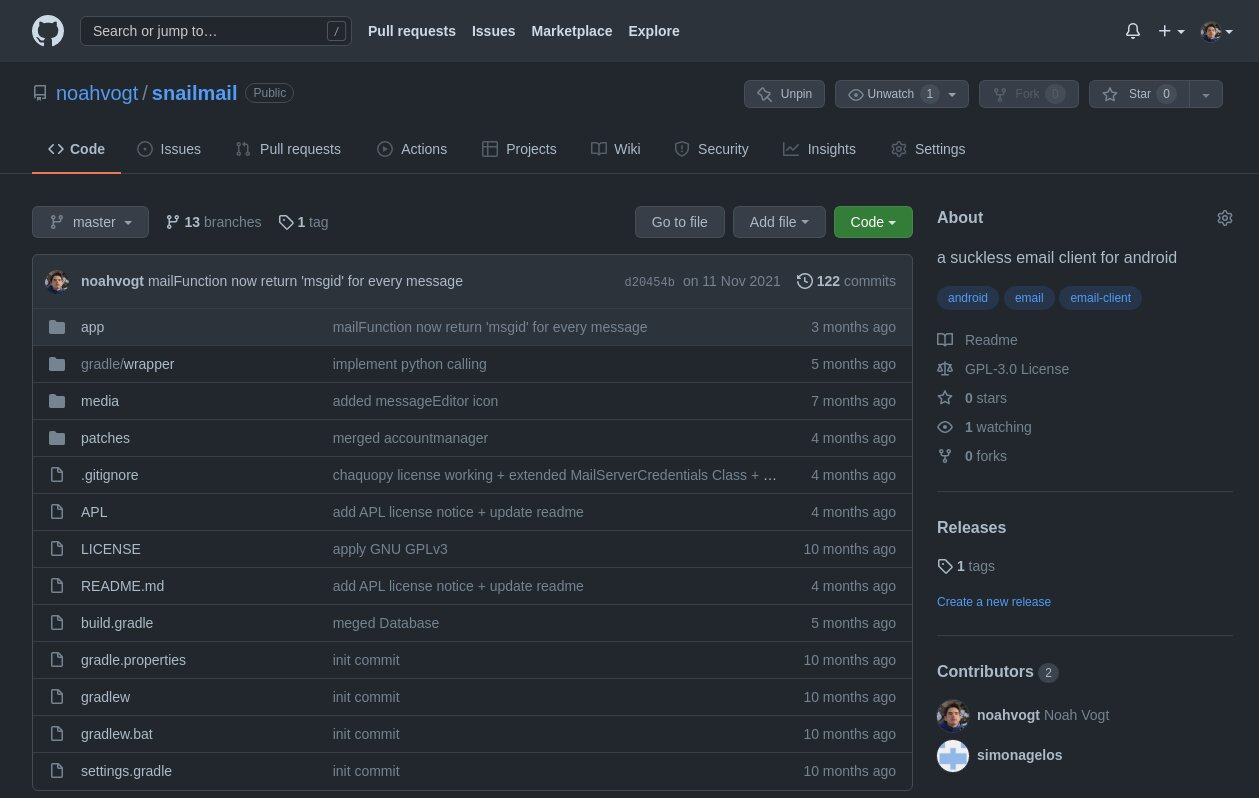
\includegraphics[height=.7\textheight]{media/github-repo.jpg}
    \end{figure}
    \begin{itemize}
        \centering
        \item https://github.com/noahvogt/snailmail
        \item https://git.noahvogt.com/me/snailmail
    \end{itemize}
\end{frame}

\end{document}
